\documentclass[journal,12pt,onecolumn]{IEEEtran}
\usepackage[utf8]{inputenc}   % Codificación de entrada
\usepackage[T1]{fontenc}      % Codificación de fuente
\usepackage[spanish,es-tabla]{babel}   % Idioma español
\usepackage{lmodern}          % Fuente moderna
\usepackage{amsmath, amssymb} % Matemáticas y símbolos
\usepackage{graphicx} 		  % Gráficos e imágenes
\graphicspath{{img/}{tablas/}{portada/}}  % Las imágenes se buscarán en la carpeta "img"
\usepackage{longtable}      % Para tablas que se extienden en varias páginas
\usepackage{tabularx}	% Tablas avanzadas
\usepackage{threeparttable}
\usepackage{hyperref}	% Hipervínculos

%-------------------------------------------
% Otros paquetes útiles (personaliza según tus necesidades)
%-------------------------------------------
\usepackage{caption}
\usepackage{subcaption}
\usepackage{xcolor}
\usepackage{setspace}

%-------------------------------------------
% Comandos personalizados
\renewcommand{\listtablename}{Índice de tablas}
\renewcommand{\appendixname}{Anexos}
\definecolor{colorreferences}{RGB}{48,134,3}

% Metadatos del PDF
\hypersetup{
	unicode=true,
	hidelinks,
	colorlinks=true,       % false: boxed links; true: colored links
	linkcolor=black,          % color of internal links (change box color with linkbordercolor)
	citecolor=colorreferences,        % color of links to bibliography
	filecolor=magenta,      % color of file links
	urlcolor=blue,           % color of external links
	linkbordercolor={0 0 0}
}
%-------------------------------------------
% Inicio del documento
%-------------------------------------------
\begin{document}

% Aquí se encuentra el archivo con la portada
\begin{titlepage}
	\centering
	%-------------------------------------------
	% Logos en una tabla: izquierda, centro y derecha
	\begin{tabular}{@{}p{0.3\textwidth} p{0.3\textwidth} p{0.3\textwidth}@{}}
		
\includegraphics[height=2cm]{tecnm} & 
		\centering 
\includegraphics[height=1.5cm]{SEP} & 
		\raggedleft 
\includegraphics[height=2cm]{ith.jpg} \\
	\end{tabular}
	
	\vspace{2em}
	
	\noindent
	%-------------------------------------------
	%	Información institucional y académica (esquina superior izquierda)
	\begin{minipage}[t]{0.6\textwidth}
		\raggedright
		\small \textbf{%
			Instituto Tecnológico de Hermosillo\\
			Materia: Robótica\\
			Profesor: Medina Gil Lamadrid, Jesús Iván%
		}
	\end{minipage}%
	\hfill
	%	fecha actual (esquina superior derecha), en letras pequeñas y en negrita.
	\begin{minipage}[t]{0.3\textwidth}
		\raggedleft
		\small \textbf{\today}
	\end{minipage}
	
	\vspace{2em}
	
	%-----------------------------------------
	% Unidad y Título de la tarea en letras grandes y en negrita
%	{\large \textbf{Unidad Final}}\\
	{\Huge \textbf{Reporte final del Robot}}
		
	\vspace{1em}
	
	%---------------------------------------
	% Tabla con la información del equipo
	%---------------------------------------
	% Encabezado del equipo
	\begin{center}
		{\Large \textbf{Equipo N}}
		
		{\small \textbf{https://github.com/DueñoDelRepositorio/Robotica.git}}
	\end{center}
	
	\vspace{1em}
	
	% Tabla de integrantes:
	% Cada fila contiene: foto (columna izquierda) y datos del integrante (columna derecha)
	\begin{center}
		\begin{tabular}{c c}
			\begin{tabular}{c}
				
\includegraphics[height=3cm]{perfil1.jpg} \\
				\textbf{Apellido1},\\ Nombre1 \\ \texttt{correo1@ejemplo.com} \\ Teléfono: (opcional)
			\end{tabular} &
			\begin{tabular}{c}
				
\includegraphics[height=3cm]{perfil2.jpg} \\
				\textbf{Apellido2,}\\ Nombre2 \\ \texttt{correo2@ejemplo.com} \\ Teléfono: (opcional)
			\end{tabular} \\ \vspace{2em}
			\begin{tabular}{c}
				
\includegraphics[height=3cm]{perfil3.jpg} \\
				\textbf{Apellido3,}\\ Nombre3 \\ \texttt{correo3@ejemplo.com} \\ Teléfono: (opcional)
			\end{tabular} &
			\begin{tabular}{c}
				
\includegraphics[height=3cm]{perfil4.jpg} \\
				\textbf{Apellido4,}\\ Nombre4 \\ \texttt{correo4@ejemplo.com} \\ Teléfono: (opcional)
			\end{tabular}
		\end{tabular}
	\end{center}

\end{titlepage}

%	Es innecesario poner el índice porque ya aparece en los marcadores del PDF
%\tableofcontents

% Ejemplo de inclusión de una sección (por ejemplo, "introduccion.tex" debe estar en la carpeta "secciones" y se recomienda no usar carácteres especiales (tilde) o espacios)
\section{Introducción}
\LaTeX es una herramienta poderosa para la creación de documentos técnicos y científicos, permitiendo la generación de contenido con alta calidad tipográfica. En este documento se han explorado diferentes aspectos fundamentales para la creación de reportes en \LaTeX, incluyendo la inserción de imágenes, la organización de tablas y la formulación de ecuaciones matemáticas.

Algo que se puede dar a notar es que las secciones tienen nombres un pcoo diferentes a los que están acostumbrados. Les doy libertad para usar nombres libres o usar nombres clásicos, como marco teórico. También pueden usar una sección llamada marco teórico y subsecciones más específicas como puse en la \autoref{sec:conclusion}: Conclusión.

Aun hay muchas cosas que no se abarcaron en este documento, pero pueden preguntarle a chatGPT, a Deepseek o simplemente googlearlo. 

\section{Sensores Internos}

Ya que un robot industrial maneja altos niveles de precisión, velocidad e inteligencia, es necesario que este cuente con el conocimiento en relación con su propio funcionamiento; de ahí la vital importancia de sus sensores internos, pues estos serán aquellos que nos confirmen:
    \begin{itemize}
        \item El estado de sus propias articulaciones.
        \item El monitoreo de sus posiciones, velocidades y aceleraciones.
    \end{itemize}
Ya que basado en esta información, el operador o controlador podrá tomar decisiones sobre los diferentes comandos, tanto preventivos como de reacción.

\section{Sensores Internos de posicion}
\subsection{Codificadores angulares de posición (encoders)}

Los codificadores ópticos o encoders incrementales constan, en su forma más simple, de un disco transparente con una serie de marcas opacas colocadas radialmente y equidistantes entre sí; de un sistema de iluminación en el que la luz es colimada de forma correcta, y de un elemento fotorreceptor. El eje cuya posición se quiere medir va acoplado al disco transparente. Con esta disposición, a medida que el eje gira se irán generando pulsos en el receptor cada vez que la luz atraviese cada marca, y llevando una cuenta de estos pulsos es posible conocer la posición del eje.



\begin{figure}[h]
	\centering
	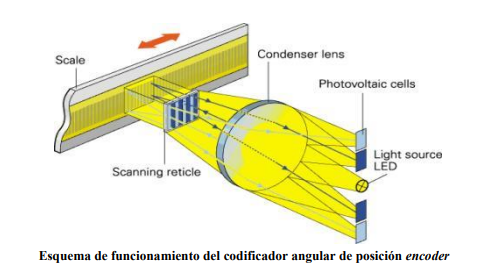
\includegraphics[width=0.7\linewidth]{img/codificador angular de posicion.png}
	\caption{Codificador angular de posicion}
	\label{fig:insertarimagen}
\end{figure}

El funcionamiento básico de los codificadores o encoders absolutos es similar al de los incrementales. Se tiene una fuente de luz con las lentes de adaptación correspondientes, un disco graduado y unos fotorreceptores. En este caso, el disco transparente se divide en un número determinado de sectores (potencia de 2), codificándose cada uno de ellos según un código binario cíclico (normalmente código de Gray) que queda representado por zonas transparentes y opacas dispuestas radialmente. No es necesario ahora ningún contador o electrónica adicional para detectar el sentido del giro, pues cada posición (sector) es codificado de forma absoluta. Su resolución es fija, y vendrá dada por el número de anillos que posea el disco graduado. Las resoluciones habituales van desde 28 a 219 bits (desde 256 a 524288 posiciones distintas)

Normalmente los sensores de posición se acoplan al eje del motor. Considerando que en la mayor parte de los casos entre el eje del motor y el de la articulación se sitúa un reductor de relación N, cada movimiento de la articulación se verá multiplicado por N al ser medido por el sensor. Éste aumentara así su resolución, multiplicándola por N.

\begin{figure}[h]
	\centering
	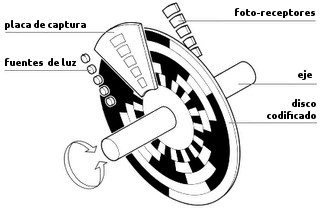
\includegraphics[width=0.7\linewidth]{img/codificador angular 2.jpg}
	\caption{Codificador angular de posicion}
	\label{fig:insertarimagen}
\end{figure}

\subsection{Codificadores angulares de posición (sincro-resolvers)}

La otra alternativa en sensores de posición para robots la representan los resolvers y los sincroresolvers, también llamados sincros. Se trata de sensores analógicos con resolución teóricamente infinita. El funcionamiento de los resolvers se basa en la utilización de una bobina solidaria al eje excitada por una portadora, generalmente con 400Hz, y por dos bobinas fijas situadas a su alrededor.

\begin{figure}[h]
	\centering
	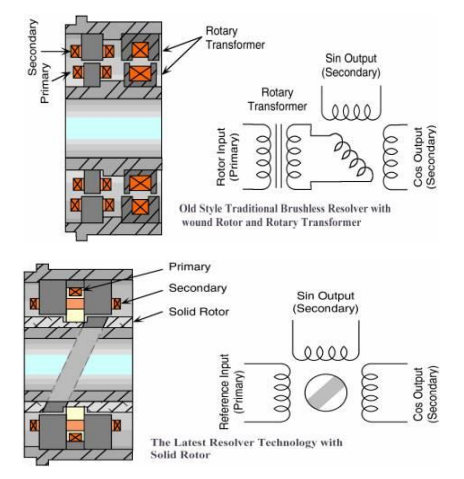
\includegraphics[width=0.7\linewidth]{img/sincroresolvers 1.png}
	\caption{sincroresolver}
	\label{fig:insertarimagen}
\end{figure}



El giro de la bobina móvil hace que el acoplamiento con las bobinas fijas varía, consiguiendo que la señal resultante en éstas dependa del seno del ángulo de giro. La bobina móvil excitada con tensión V sen(wt) y girada un ángulo Ø induce en las bobinas fijas situadas en cuadratura las siguientes tensiones:

 V1= V sen(wt) sen Ø
 V2 = V sen(wt) cos Ø 
 
que es llamada representación del ángulo Ø en formato sincro. El cambio del llamado formato sincro a formato resolver o viceversa es inmediato, ya que se puede pasar de uno a otro a través de la llamada red de Scott, o transformador de Scott, o funcionamiento bidireccional. Para poder tratar el sistema de control, la información generada por los resolvers y los sincros es necesario convertir las señales analógicas en digitales. Para ello se utilizan los llamados convertidores resolver/digital (r/d), que tradicionalmente se basan en dos tipos de estructuras distintas: traking y muestreo (sampling).


Ambos captadores son del tipo absoluto en cada vuelta del eje acoplado a ellos. Entre sus ventajas destacan su buena robustez mecánica durante el funcionamiento y su inmunidad a contaminación, humedad, altas temperaturas y vibraciones. Debido a su reducido momento de inercia, imponen poca carga mecánica del funcionamiento del eje.

\subsection{Sensores lineales de posición (LVDT)}

Entre los sensores de posición lineales destaca el transformador diferencial de variación lineal (LVDT) debido a su casi infinita resolución, poco rozamiento y alta repetibilidad. Su funcionamiento se basa en la utilización de un núcleo de material ferromagnético unido al eje cuyo movimiento se quiere medir. Este núcleo se mueve linealmente entre un devanado primario y dos secundarios, haciendo con su movimiento que varíe la inductancia entre ellos.
Los dos devanados secundarios conectados en oposición serie ven como la inducción de la tensión alterna del primario, al variar la posición del núcleo, hace crecer la tensión de un devanado y disminuir la del otro. Del estudio de la tensión se deduce que ésta es proporcional a la diferencia de inductancias mutuas entre el devanado primario con cada uno de los secundarios, y que por tanto depende linealmente del desplazamiento del vástago solidario al núcleo.
 Además de las ventajas señaladas, el LVDT presenta una alta linealidad, gran sensibilidad y una respuesta dinámica elevada. Su uso está ampliamente extendido, a pesar del inconveniente de poder ser aplicado únicamente en la medición de pequeños desplazamientos.

\begin{figure}[h]
	\centering
	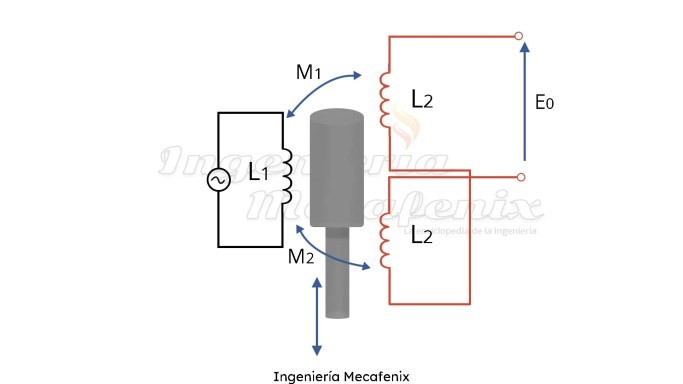
\includegraphics[width=0.7\linewidth]{img/sensor posicion.jpg}
	\caption{Codificador angular de posicion}
	\label{fig:insertarimagen}
\end{figure}

\subsection{Sensores lineales de posición (potenciómetro)}

Los sensores de posición potenciométricos, también llamados sensores resistivos, miden la resistencia de una pista conductora entre un punto de referencia y un cursor conectado a una pieza móvil —o a su soporte—. La resistencia medida por el sensor permite calcular la posición de la pieza.
Estos sensores suelen ser económicos ya que su tecnología es sencilla y precisa. Sin embargo, a menudo se ven afectados por el desgaste, las vibraciones, los cuerpos extraños y las temperaturas extremas.

\begin{figure}[h]
	\centering
	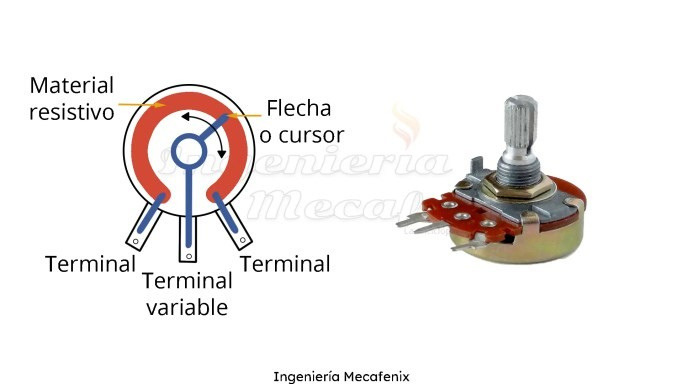
\includegraphics[width=0.7\linewidth]{img/potenciometro.jpg}
	\caption{potenciometro}
	\label{fig:insertarimagen}
\end{figure}

Puntos fuertes:

\begin{itemize}
    \item Tecnología sencilla.
    \item Medición precisa.
    \item Precio económico
    \item 
\end{itemize}

\section{Sensores Internos de velocidad}

\subsection{Efecto Hall }

Un sensor de efecto Hall mide los cambios en el campo magnético del imán, causados por el material objetivo ferromagnético. Los sensores tienen acondicionadores de señal incorporados, que generan una señal de onda cuadrada clara. A diferencia de los sensores VR, los sensores de efecto Hall son sensibles al tamaño del flujo magnético y no a la velocidad a la que cambia. Los sensores de velocidad de efecto Hall tienen un amplio rango de medición y pueden utilizarse para medir tanto piezas de baja velocidad o estacionarias como piezas de alta velocidad.

Ventajas:
Una ventaja de un sensor de efecto Hall es que el sensor proporciona directamente una salida digital que es fácil de transmitir y procesar. Otra ventaja es que los sensores de efecto Hall suelen contar con un procesamiento interno de la señal. La señal se digitaliza y amplifica, lo que la hace menos susceptible a las interferencias electromagnéticas (EMI).
Desventajas:
Debido a la electrónica incorporada, los sensores de efecto Hall están limitados a aplicaciones que funcionan a temperaturas que van de -40 °C a +150 °C. Además, los sensores de efecto Hall requieren una conexión de 3 hilos. Asimismo, el nivel de activación se define en el sensor de efecto Hall y no puede modificarse.

\begin{figure}[h]
	\centering
	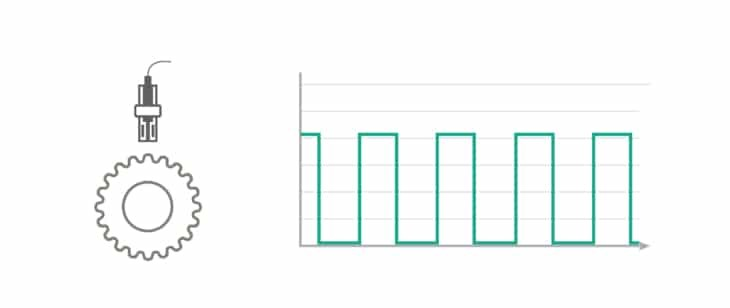
\includegraphics[width=0.7\linewidth]{img/efecto hall.jpg}
	\caption{Sensor efecto hall}
	\label{fig:insertarimagen}
\end{figure}

Un sensor de efecto Hall genera una señal de salida de onda cuadrada.

\begin{figure}[h]
	\centering
	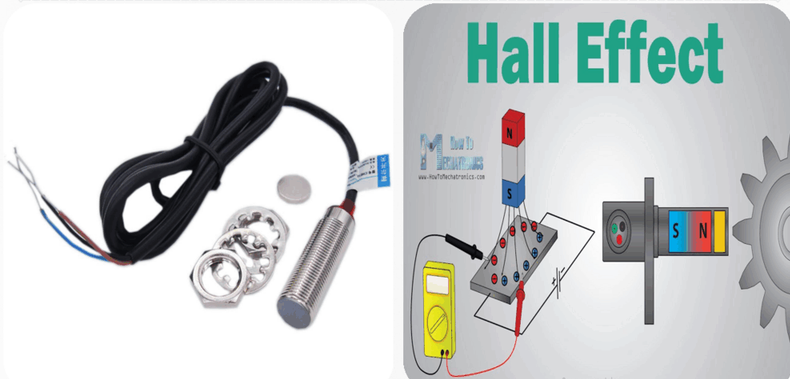
\includegraphics[width=0.7\linewidth]{img/sensor efecto hall.png}
	\caption{Sensor efecto hall}
	\label{fig:insertarimagen}
\end{figure}

\subsection{tacometro }
El tacómetro es un dispositivo que mide la velocidad de rotación de un objeto. El término viene del griego “táchos” que significa velocidad y, de la palabra “metron” que significa medida. En un vehículo, se encarga de medir la velocidad de rotación del eje del motor marcando las revoluciones por minuto (RPM), es decir, la velocidad a la que gira el motor del vehículo.
Un tacómetro está formado por un dial, una aguja para indicar la lectura en tiempo real y unas marcas para identificar cuáles son los niveles seguros de velocidad y cuáles son aquellos que significan un peligro.
En sus inicios, el tacómetro medía la fuerza centrífuga y no la fuerza lineal, eran dispositivos mecánicos. En la actualidad, los tacómetros son digitales y más precisos.
El tacómetro en los vehículos determina la velocidad del eje de transmisión del motor, es decir, informa al conductor cuando debe cambiar de marcha para no forzar el motor y alargar su vida útil. La forma en la que se realizan estas mediciones puede variar:
Desde un generador
Los motores con sistemas de encendido por lo general usan un generador conectado al eje de transmisión del motor, por lo tanto, más que un tacómetro es un voltímetro o medidor de tensión, lo cual quiere decir que mide las pulsaciones de tensión en el sistema de encendido. El voltaje de salida es proporcional a la velocidad del eje por tanto la medición de tensión se convierte en una medición precisa en revolución por minuto (RPM).

Desde las chispas
Se trata de un método simple, pero muy poco común, se mide la velocidad a la que se liberan las chispas en los cilindros del motor. Es una acción que solo se observa en los motores de gasolina, porque en estos es habitual el uso de bujías, estas son las encargadas de brindar la energía calorífica que mueve el coche.

Desde un láser
El tacómetro láser es uno de los más populares en la actualidad, debido a que no necesita contacto con el eje del motor, sino que trabaja mediante una luz infrarrojo hacia el eje. Este tipo de tacómetro mide el ritmo mediante el cual se refleja la luz de vuelta en el tacómetro.

Tipos de tacómetros
Podemos hablar de dos tipos de tacómetros:
Analógicos: constituidos por una aguja y un dial de interfaz, realizando el marcaje de la velocidad con un disco cuentakilómetros para finalmente marcarlo en la pantalla. Tal y como se tratará de un reloj.

\begin{figure}[h]
	\centering
	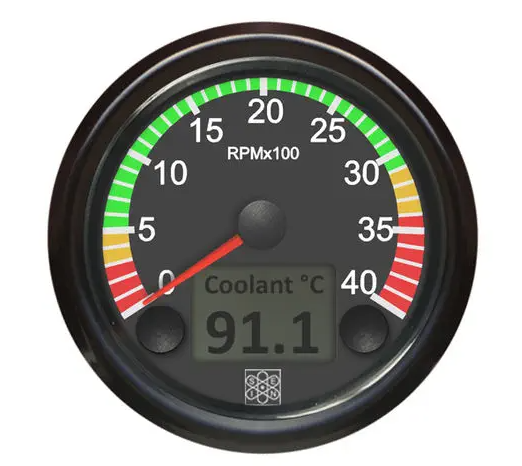
\includegraphics[width=0.7\linewidth]{img/tacometro.png}
	\caption{Tacometro}
	\label{fig:insertarimagen}
\end{figure}

Digitales: constituidos por una pantalla LCD o LED y una memoria para el almacenamiento, proporcionando lecturas numéricas en lugar de usar cuadrantes y agujas

Partes de un tacómetro: 
\begin{itemize}
    \item Imán: la parte más importante del tacómetro, permite cumplir con todo el funcionamiento, mediante un campo magnético para realizar los marcajes.
    \item Muelle espiral: permite amortiguar la torsión con forma espiral.
    \item Órgano de transmisión: transmite los datos obtenidos en la rotación del imán.
    \item Tornillo sin fin: comunica el movimiento que hay entre los ejes.
    \item Árbol de accionamiento: unión entre el sector de accionamiento del motor con el cambiador de las tomas.
    \item Anillos: cuenta con varios anillos, pero el más importante es el arrastrado por el campo magnético del imán para hacer el marcaje en la pantalla.
    \item Pantalla: la información que se desglosa en el disco del salpicadero del coche, mediante unidades kilométricas, una aguja y una escala.
    \item 
\end{itemize}

\section{Sensores de aceleracion}
Los acelerómetros miden la aceleración lineal de un objeto en una o varias direcciones.

\subsection{Acelerómetros mecánicos: }
Los acelerómetros mecánicos son sensores que detectan la aceleración utilizando principios mecánicos, como masas móviles, resortes y amortiguadores. Son algunos de los tipos más antiguos de acelerómetros y se siguen utilizando en aplicaciones donde la robustez y la simplicidad son clave.

\begin{figure}[h]
	\centering
	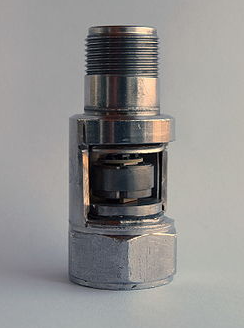
\includegraphics[width=0.7\linewidth]{img/acelerometro.png}
	\caption{Acelerometro}
	\label{fig:insertarimagen}
\end{figure}

\subsection{Acelerómetros piezoeléctricos }

Este tipo de dispositivo hace uso del efecto piezoeléctrico. ordinariamente, hay una masa adherida a un cristal piezoeléctrico. Cuando hay una aceleración en el sistema, la masa adherida al cristal termina generando una deformación y este desplazamiento genera una señal eléctrica.
La solución a los problemas de los acelerómetros resistivos más antiguos., resultado de la introducción del acelerómetro piezoeléctrico. Los materiales piezoeléctricos utilizados tienen una alta rigidez. Además, sus respuestas eléctricas autogeneradas produjeron amplios rangos de señal dinámica. Ambas propiedades combinadas permiten el diseño de acelerómetros con altas frecuencias de resonancia. Estas altas frecuencias de resonancia han eliminado la necesidad de amortiguación para aumentar la respuesta de frecuencia plana utilizable del acelerómetro. También se ha eliminado el cambio de fase en el rango de frecuencia utilizable del acelerómetro. Este gran rango de señal dinámica también permitió la reducción del tamaño de los acelerómetros piezoeléctricos en comparación con los acelerómetros de galgas extensométricas., al tiempo que proporciona la capacidad de medir aceleraciones mucho mayores.

\begin{figure}[h]
	\centering
	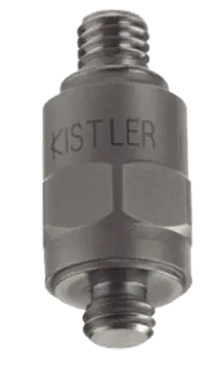
\includegraphics[width=0.5\linewidth]{img/Acelerometro piezoelectrico.png}
	\caption{Acelerometro piezoelectrico}
	\label{fig:insertarimagen}
\end{figure}


\subsection{Acelerómetros MEMS (Microelectromechanical Systems): }
Hoy en día, en muchas aplicaciones, se utilizan acelerómetros fabricados con tecnología MEMS ("sistemas micro electromecánicos").
Esta técnica crea estructuras de detección mecánica de tamaño microscópico, generalmente en silicio. Cuando se acopla a circuitos microelectrónicos, Los sensores MEMS se pueden utilizar para medir parámetros físicos, como aceleración
Entonces, más que un solo tipo de acelerómetro, es una técnica de fabricación de acelerómetros.
Básicamente consisten en una estructura incorporada con una masa. Bajo la influencia de una aceleración externa, la estructura se deforma., por el efecto de la fuerza ejercida por la masa, y esta deformación se mide permitiendo conocer la aceleración.
La forma de medir la deformación puede ser diferente. Hoy en día existen tipos de acelerómetros MEMS, resistivos, capacitivos, servo acelerómetros, etc.

\begin{figure}[h]
	\centering
	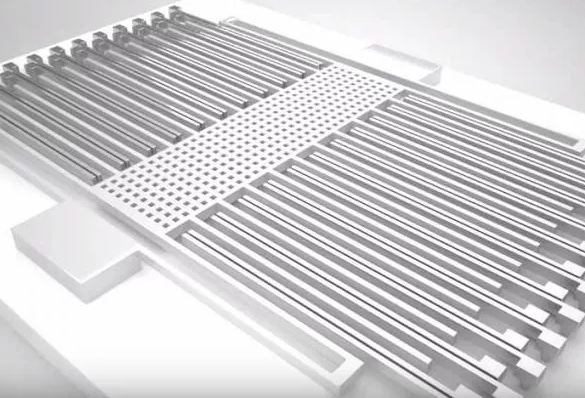
\includegraphics[width=0.7\linewidth]{img/acelerometros MEMS.png}
	\caption{Acelerometro MEMS}
	\label{fig:insertarimagen}
\end{figure}

\subsection{Acelerómetros capacitivos}

Un acelerómetro capacitivo funciona de modo que la aceleración en el dispositivo desplaza una placa móvil de un condensador en relación con las placas fijas del dispositivo. de esta, cómo cambia la capacitancia de cada condensador.
Acelerómetros capacitivos, dependen de un cambio en la capacitancia eléctrica en respuesta a la aceleración. Los acelerómetros utilizan las propiedades de un condensador de placa opuesta, para el cual la distancia entre las placas varía en proporción a la aceleración aplicada, cambiando así la capacitancia. Esta variable se utiliza en un circuito para proporcionar una señal de voltaje proporcional a la aceleración.
Los acelerómetros capacitivos son capaces de medir aceleraciones periódicas y transitorias constantes, desde DC. Los sensores de aceleración capacitiva de CA contienen fundamentalmente al menos dos componentes; el primario es un tablero “estacionario” (esto es, conectado a la vivienda) y la placa secundaria se fija a la masa inercial, quién es libre de moverse dentro de la vivienda. Estas placas forman un condensador cuyo valor es función de la distancia d entre las placas. El material de detección es una placa plana de níquel o un chip electrónico soportado sobre la superficie del sustrato por dos barras de torsión unidas a un pedestal central. Un acelerómetro capacitivo rara vez excede un desplazamiento máximo de 20 μm. por lo tanto, un desplazamiento tan pequeño requiere una medición fiable de las desviaciones y diversas interferencias. Cuando se somete a aceleración fija o constante, el valor de capacitancia también es constante., dando como resultado una señal de medición proporcional a la aceleración uniforme, también conocido como DC o aceleración estática.



\begin{figure}[h]
	\centering
	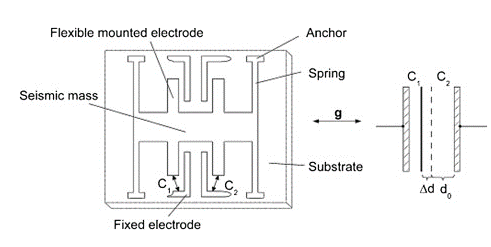
\includegraphics[width=0.7\linewidth]{img/acelerometro capacitivo.png}
	\caption{Acelerometro capacitivo}
	\label{fig:insertarimagen}
\end{figure}

Características típicas:
\begin{itemize}
    \item Suelen proporcionar buenas especificaciones térmicas. -54 una + 121 ºC
    \item Capacidad de respuesta DC
    \item Distancia:  +/- 2 una 200 Gs FS
    \item Gran capacidad por encima del rango (por ejemplo, 5.000 Gs)
    \item Generalmente proporciona +/- 2 voltios de potencia CC no regulados
    \item Aplicaciones Típicas: transporte, aleteo de aeronaves
\end{itemize}

\subsection{Acelerómetros optico}

El acelerómetro de fibra óptica MEMS (FOA) de Sercalo es un sensor de aceleración opto-mecánico. El dispositivo de detección es un espejo de silicio micromecánico (MEMS) que desvía un haz de luz proporcional a la aceleración. Puede colocarse en un entorno hostil y está separado de la electrónica de medición mediante fibras ópticas.
Los acelerómetros ópticos son un tipo de acelerómetro que utiliza luz para medir la aceleración. Por lo general, están hechos de silicio u otros materiales semiconductores y utilizan interferometría para medir los pequeños cambios en la distancia entre dos espejos causados por la aceleración. Nuestros acelerómetros ópticos ofrecen varias ventajas sobre los acelerómetros tradicionales, entre ellas, alta precisión, bajo nivel de ruido y amplio ancho de banda.


\begin{figure}[h]
	\centering
	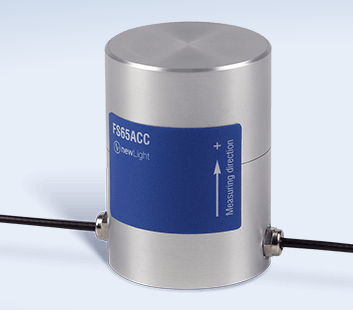
\includegraphics[width=0.7\linewidth]{img/acelerometro optico.png}
	\caption{Acelerometro optico}
	\label{fig:insertarimagen}
\end{figure}

\section{Sensores de fuerza}
\subsection{Galgas Extensométricas.}

Las galgas extensiométricas son sensores cuya resistencia varía con la fuerza aplicada. Estos sensores convierten la fuerza, presión, tensión, peso, etc, en un cambio de la resistencia eléctrica el cual puede ser medido.
Este tipo de sensores son los elementos más importantes en el diseño de transductores de presión y células de carga. La correcta utilización de las galgas para medir fuerzas y deformaciones es una de las herramientas más importantes en la ingeniería o la construcción.

\subsection{Interruptores de Efecto Hall.}

Los interruptores de efecto Hall son dispositivos electrónicos que utilizan campos magnéticos para detectar las pulsaciones de teclas. A diferencia de los interruptores mecánicos, dependen de campos magnéticos en lugar del contacto físico.

Esto da como resultado menos piezas móviles, lo que a menudo conduce a una mayor durabilidad y confiabilidad.
El principio detrás de los interruptores de efecto Hall fue descubierto por el físico Edwin Hall en 1879. Implica medir la diferencia de voltaje a través de un conductor por el que se aplica un campo magnético.
La presencia de un campo magnético hace que la carga eléctrica se vea afectada, permitiendo que el interruptor detecte cambios.
Aplicaciones.
Interruptores de teclado: se utilizan en algunos teclados para lograr una experiencia de escritura fluida.
Controles industriales: se emplean en maquinaria donde la durabilidad es crucial.
Automotriz: Se encuentra en vehículos para funciones como cambios de marcha y sensores.
Ventajas:
Resistente al polvo y a la humedad: esta característica los hace adecuados para entornos hostiles.
Funcionamiento suave: elimina la sensación táctil de los interruptores mecánicos tradicionales.



\begin{figure}[h]
	\centering
	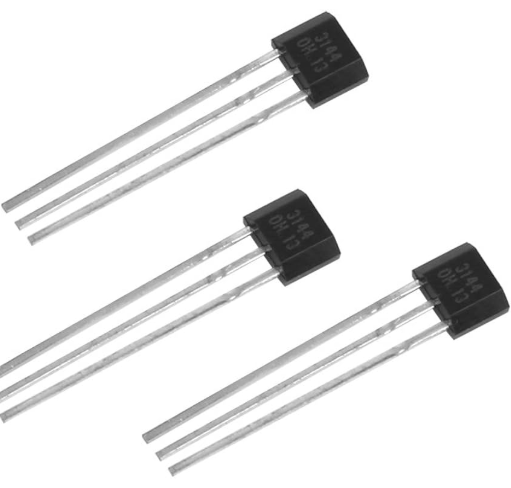
\includegraphics[width=0.7\linewidth]{img/int ef hall.png}
	\caption{interruptores efecto hall}
	\label{fig:insertarimagen}
\end{figure}

\subsection{Interruptores piezoelectricos.}

También conocido como interruptor piezoeléctrico, un interruptor piezoeléctrico es un tipo relativamente nuevo de interruptor eléctrico que se caracteriza por su método de funcionamiento piezoeléctrico. Puede encontrarlos en teclados, interfaces hombre-máquina (HMI) y otros dispositivos de entrada basados en circuitos. Interruptores piezoeléctricos disponen de uno o varios botones que, al pulsarlos, abren o cierran el circuito correspondiente.
Aunque hay muchos tipos de interruptores piezoeléctricos, todos utilizan el mismo método de funcionamiento. Para que un interruptor se considere piezoeléctrico, debe utilizar un elemento piezoeléctrico. El elemento piezoeléctrico es el responsable de generar una tensión que abre o cierra el circuito correspondiente. Al pulsar un botón, el elemento piezoeléctrico generará una tensión. Esta tensión abrirá o cerrará el circuito correspondiente.

Los elementos piezoeléctricos son componentes que generan una tensión en respuesta a una tensión mecánica. Al pulsar un botón se crea una tensión mecánica. Esta tensión mecánica apretará esencialmente el elemento piezoeléctrico para que genere electricidad, que a su vez abre o cierra el circuito correspondiente.

\begin{figure}[h]
	\centering
	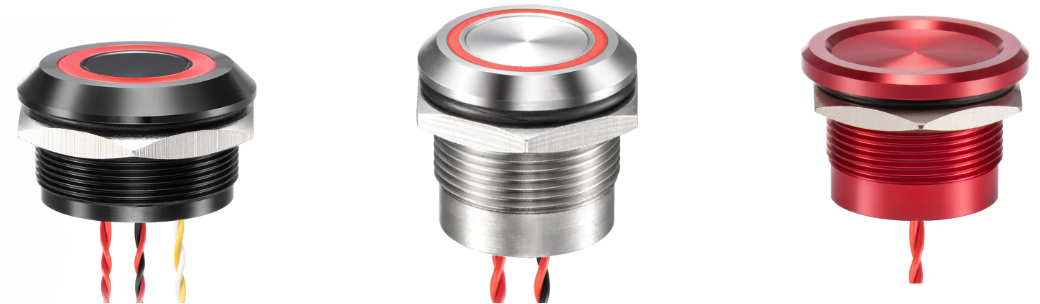
\includegraphics[width=0.7\linewidth]{img/int piezoelectrico.png}
	\caption{interruptores piezoelectrico}
	\label{fig:insertarimagen}
\end{figure}

\section{Sensores Externos}
\section{tipo contacto}
\subsection{Interruptores de limite}
Son dispositivos electromecánicos que se activan cuando un objeto hace contacto con su palanca o botón. Suelen utilizarse en maquinaria industrial para detectar la posición de piezas móviles o detener un proceso cuando se alcanza un límite seguro.
Ejemplo: En una banda transportadora un interruptor de límite puede detectar cuando un producto llega al final del recorrido deteniendo la máquina para evitar acumulaciones.


\begin{figure}[h]
	\centering
	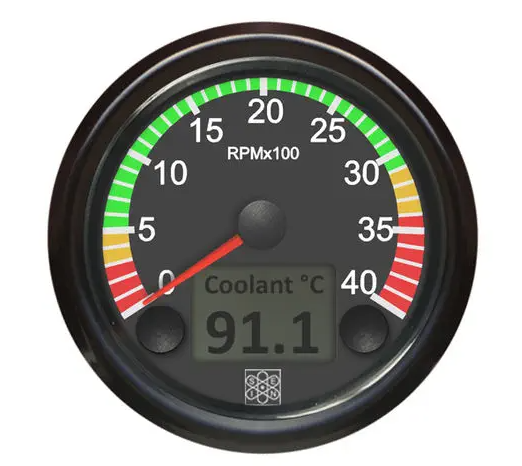
\includegraphics[width=0.7\linewidth]{img/tacometro.png}
	\caption{Tacometro}
	\label{fig:insertarimagen}
\end{figure}
\subsection{Interruptores neumáticos:}
Funcionan mediante la presión de aire sin necesidad de componentes eléctricos lo que los hace ideales para ambientes donde las chispas eléctricas podrían representar un peligro. Se usan en aplicaciones industriales donde se requiere una detección segura y confiable.
Ejemplo: En una prensa neumática un interruptor de este tipo puede asegurarse de que la pieza esté correctamente colocada antes de iniciar el proceso de prensado.

\begin{figure}[h]
	\centering
	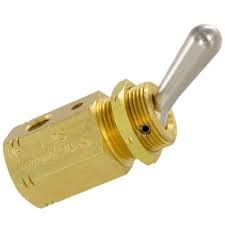
\includegraphics[width=0.7\linewidth]{img/interruptor neumatico.jpg}
	\caption{interruptor neumatico}
	\label{fig:insertarimagen}
\end{figure}

\subsection{Sensores piezoeléctricos: }
Aprovechan el efecto piezoeléctrico en el cual ciertos materiales generan una carga eléctrica cuando se les aplica presión mecánica. Son ampliamente usados en medición de vibraciones impacto y presión.
Ejemplo: En un motor industrial un sensor piezoeléctrico puede monitorear vibraciones anormales para detectar fallos antes de que ocurran.


\begin{figure}[h]
	\centering
	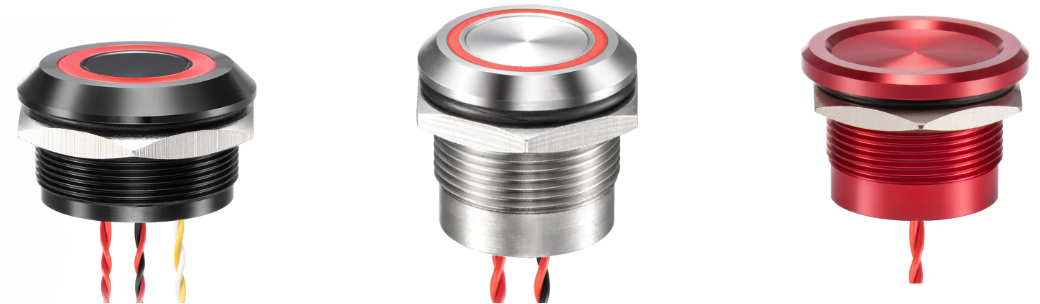
\includegraphics[width=0.7\linewidth]{img/int piezoelectrico.png}
	\caption{interruptores piezoelectrico}
	\label{fig:insertarimagen}
\end{figure}

\subsection{Transductores }
Son dispositivos que convierten una forma de energía en otra permitiendo la medición de distintas magnitudes físicas como presión temperatura o sonido. Son utilizados en diversas industrias para monitoreo y control.
Ejemplo: Un transductor de presión en un sistema hidráulico convierte los cambios de presión en señales eléctricas que pueden ser interpretadas por un sistema de control.


\begin{figure}[h]
	\centering
	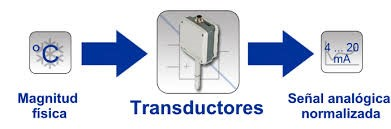
\includegraphics[width=0.7\linewidth]{img/transductor.jpg}
	\caption{transductor}
	\label{fig:insertarimagen}
\end{figure}

\section{tipo sin contacto}
\subsection{Sensores de proximidad:  }
Detectan la presencia de un objeto sin necesidad de contacto físico. Pueden basarse en tecnologías como ultrasonidos infrarrojos o campos electromagnéticos. Son comunes en sistemas automatizados y en robótica.
Ejemplo: En una línea de ensamblaje un sensor de proximidad puede verificar si una pieza está en la posición correcta antes de continuar con el siguiente paso del proceso.

\begin{figure}[h]
	\centering
	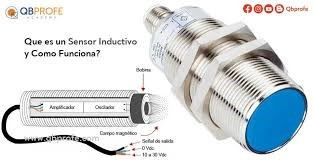
\includegraphics[width=0.7\linewidth]{img/sensor de proximidad.jpg}
	\caption{Sensor de proximidad}
	\label{fig:insertarimagen}
\end{figure}

\subsection{Sensores de efecto hall }
Funcionan detectando cambios en un campo magnético lo que permite determinar la posición o velocidad de un objeto metálico en movimiento. Son muy utilizados en motores eléctricos y sistemas de frenos de vehículos.
Ejemplo: En un automóvil los sensores de efecto Hall permiten medir la velocidad de las ruedas ayudando al sistema de frenos ABS a actuar de manera eficiente.


\begin{figure}[h]
	\centering
	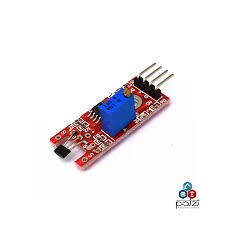
\includegraphics[width=0.7\linewidth]{img/s. efecto hall.jpg}
	\caption{Sensor efecto hall}
	\label{fig:insertarimagen}
\end{figure}

\subsection{Sensores de microondas }
Utilizan ondas electromagnéticas de alta frecuencia para detectar objetos o movimientos incluso a través de materiales no metálicos. Son muy empleados en sistemas de seguridad y control de accesos.
Ejemplo: En una puerta automática un sensor de microondas detecta la aproximación de una persona activando la apertura sin necesidad de contacto.

\begin{figure}[h]
	\centering
	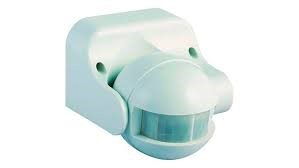
\includegraphics[width=0.7\linewidth]{img/sensor microondas.jpg}
	\caption{Sensor microondas}
	\label{fig:insertarimagen}
\end{figure}

\subsection{Sensores ultrasónicos:  }

Emiten ondas sonoras de alta frecuencia y miden el tiempo que tarda el eco en regresar permitiendo calcular distancias y detectar objetos. Son ideales para medición de nivel de líquidos y en sistemas de asistencia para estacionamiento.
Ejemplo: En un automóvil los sensores ultrasónicos detectan la cercanía de obstáculos durante las maniobras de aparcamiento alertando al conductor


\begin{figure}[h]
	\centering
	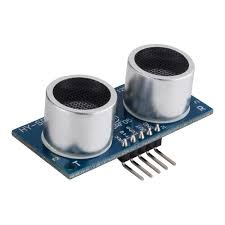
\includegraphics[width=0.7\linewidth]{img/sensor ultrasonico.jpg}
	\caption{Sensor ultrasonico}
	\label{fig:insertarimagen}
\end{figure}

\subsection{Sensores laser:  }
Utilizan un haz de luz láser para medir distancias con alta precisión. Se emplean en aplicaciones industriales donde es importante una medición exacta y rápida.

Ejemplo: En una fábrica un sensor láser puede determinar con precisión la ubicación y el tamaño de piezas en una línea de ensamblaje automatizada

\begin{figure}[h]
	\centering
	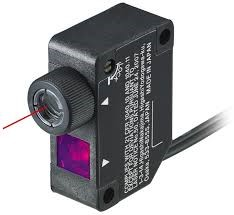
\includegraphics[width=0.7\linewidth]{img/sensor laser.jpg}
	\caption{sensor laser }
	\label{fig:insertarimagen}
\end{figure}

\subsection{Sensores de visión:  }

Sensores de visión: Capturan imágenes y las procesan para identificar objetos colores formas o patrones. Son ampliamente utilizados en sistemas de inspección de calidad y reconocimiento facial.

Ejemplo: En una fábrica de productos electrónicos un sensor de visión verifica si cada dispositivo ha sido ensamblado correctamente antes de empaquetarlo.

\begin{figure}[h]
	\centering
	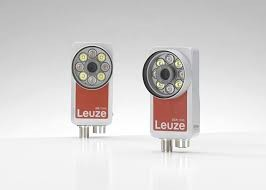
\includegraphics[width=0.7\linewidth]{img/sensor de vision.jpg}
	\caption{sensor de vision}
	\label{fig:insertarimagen}
\end{figure}

\section{giroscopio, acelerómetro, magnetómetro y LiDA. }

\subsection{  ¿Qué es un giroscopio?}


Un giroscopio, o giróscopo, es un instrumento que permite determinar la orientación de un dispositivo. Asimismo, el giroscopio también sirve para mantener o cambiar la orientación en el espacio de un dispositivo.

El giroscopio está formado por un disco que es atravesado por su eje por una barra rígida. Además, tiene un conjunto de anillas que giran alrededor del disco principal mientras éste gira alrededor de su eje.

El descubrimiento del efecto giroscópico se atribuye al alemán Johann Bohnenberger en el año 1817. No obstante, no fue hasta 1852 cuando el francés León Foucault inventó el primer giroscopio.

Una de las principales características del giroscopio es que puede girar sobre un eje sin caer. Aunque en teoría debería dejar de girar y caer, el giroscopio es capaz de mantenerse girando. 

\begin{figure}[h]
	\centering
	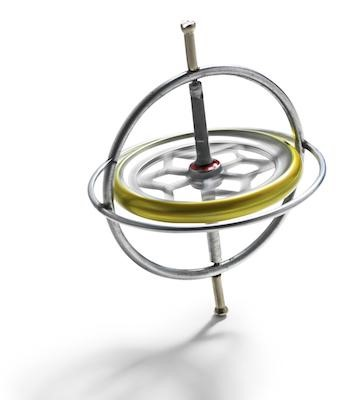
\includegraphics[width=0.7\linewidth]{img/giroscopio.jpg}
	\caption{giroscopio}
	\label{fig:insertarimagen}
\end{figure}

\subsection{ Cómo funciona un giroscopio}

Ahora que ya sabemos la definición de giroscopio, en este apartado veremos cómo funciona este dispositivo. Para entender el funcionamiento de un giroscopio primero debes saber en qué consiste el efecto giroscópico, por lo que primero se explica el efecto giroscópico y seguidamente el funcionamiento del giroscopio.

El efecto giroscópico es un fenómeno físico que sucede en los objetos con un movimiento de giro. De manera resumida, el efecto giroscópico hace que los objetos que están girando alrededor de su eje de simetría se muevan en una dirección de 90º respecto a su dirección de giro.
Así pues, el funcionamiento del giroscopio se basa en el efecto giroscópico. Cuando el giroscopio gira alrededor de su eje de simetría, aparece una fuerza que hace cambiar de orientación al giroscopio y, en consecuencia, el giroscopio no se cae y sigue girando.


\subsection{ Aplicaciones del giroscopio}

En la actualidad, el giroscopio tiene muchas utilidades y en ámbitos muy diversos. En este apartado veremos cuáles son las aplicaciones del giroscopio.

El giroscopio sirve para determinar la orientación de un objeto. Por lo tanto, las aplicaciones del giroscopio se basan en incorporar este dispositivo en objetos o vehículos para conocer su orientación.

Por ejemplo, los celulares actuales llevan incorporado un giroscopio para determinar su orientación. Así pues, el giroscopio de un celular se usa en los videojuegos para saber hacia dónde se gira el dispositivo y así interactuar con lo que está sucediendo en la pantalla del celular.

El giroscopio también se usa en los sistemas de navegación, ya que permiten saber la orientación del vehículo. Por ejemplo, en los sistemas de navegación de los aviones o de los barcos, el giroscopio es un instrumento fundamental para su funcionamiento.

Por último, las cámaras sofisticadas también tienen incorporado un giroscopio que les permite apuntar a un punto fijo mientras se están moviendo. Por ejemplo, en los deportes de acción resulta muy útil el giroscopio de la cámara, ya que de este modo se pueden hacer fotografías mientras el fotógrafo se mueve.


\subsection{ ¿Qué es un acelerómetro?}

Un acelerómetro es un instrumento que mide una aceleración. Es decir, un acelerómetro es un sensor que sirve para determinar la aceleración que experimenta un cuerpo.

Algunos acelerómetros son capaces de medir no solo la aceleración lineal de un cuerpo en los ejes X, Y y Z, sino también su aceleración angular. En consecuencia, permiten determinar la orientación del cuerpo.

Recuerda que la aceleración se define como un cambio de velocidad en el tiempo, por lo que un acelerómetro en realidad está midiendo cómo varia la velocidad.



\subsection{ Tipos de acelerómetros}

\begin{itemize}
    \item Acelerómetro mecánico: tipo de acelerómetro que mide la aceleración mediante resortes y galgas extensiométricas. Se basa en la segunda ley de Newton para calcular la aceleración.
    \item Acelerómetro capacitivo: acelerómetro que determina la aceleración midiendo el movimiento de sus capas capacitivas internas.
    \item Acelerómetro piezoeléctrico: tipo de acelerómetro que se basa en el efecto piezoeléctrico. Cuando se deforma un cristal piezoeléctrico aparece una diferencia de tensión proporcional a la fuerza aplicada, de manera que según el valor de la tensión se puede calcular la aceleración.
    \item Acelerómetro piezorresistivo: este tipo de acelerómetro es similar al acelerómetro piezoeléctrico. La resistencia de algunos materiales se ve modificada cuando se aplica una tensión, así pues, el cambio de resistencia se transforma en una señal eléctrica y con esta información se puede medir la aceleración.
    \item Acelerómetro de efecto Hall: un sensor de efecto Hall detecta los cambios magnéticos del imán del acelerómetro.
    \item 
\end{itemize}

\subsection{ Cómo funciona un acelerómetro}

En general, el funcionamiento de un acelerómetro se basa en medir la aceleración en cada uno de los tres ejes (X, Y, y Z). De este modo, se puede determinar la aceleración total del cuerpo.

Lógicamente, cada tipo de acelerómetro utiliza una manera diferente de medir. Pero normalmente los acelerómetros utilizan un mecanismo de resortes o sensores eléctricos para medir la aceleración en cada uno de los ejes. Para saber cómo funciona cada tipo de acelerómetro puedes consultar el apartado de arriba.

Además, si el cuerpo experimenta una aceleración en sentido contrario al sentido de orientación del sensor, el acelerómetro medirá la aceleración como un valor negativo. Pero si la aceleración tiene el mismo sentido que el sensor esta será positiva.

\subsection{Aplicaciones del acelerómetro}

El acelerómetro es un dispositivo que tiene muchas aplicaciones y muy diferentes, a continuación, se explican algunas de ellas:

En ingeniería, el acelerómetro tiene muchos usos. Por ejemplo, se puede utilizar un acelerómetro para medir la aceleración de un vehículo. Asimismo, el acelerómetro también se usa para determinar la vibración de una máquina o en procesos de control.
Los acelerómetros también se utilizan en biología para hacer experimentos. Por ejemplo, se puede emplear un acelerómetro para calcular el gasto calórico de un animal cuando vuela o cuando está corriendo.
Un acelerómetro también puede tener aplicaciones relacionadas con la medicina o la salud. Así pues, existen dispositivos eléctricos que miden la velocidad y la distancia recorrida por un corredor mediante un acelerómetro.
En el estudio de estructuras tiene muchas utilidades el acelerómetro, ya que permite medir el impacto de colisiones y algunos tipos de cargas difíciles de determinar, como la carga del viento.
Actualmente, los teléfonos móviles inteligentes suelen llevar incorporado un acelerómetro para poder hacer cálculos relacionados con el movimiento del smartphone.

\subsection{Diferencias entre un giroscopio y un acelerómetro}

Para terminar, veremos cuál es la diferencia entre un giroscopio y un acelerómetro, ya que son dos instrumentos que pueden complementarse y que, además, suelen confundirse.

Un acelerómetro es un instrumento que mide una aceleración. Es decir, un acelerómetro es un sensor que sirve para determinar la aceleración que experimenta un cuerpo.

Por lo tanto, la diferencia entre un giroscopio y un acelerómetro es que el giroscopio mide la orientación y la rotación del cuerpo, en cambio, el acelerómetro mide la aceleración lineal de un cuerpo.

Por esta razón, se suele utilizar la información captada por estos dos tipos de sensores de manera conjunta para hacer cálculos, ya que se complementan muy bien. Por ejemplo, los celulares suelen llevar incorporado un acelerómetro y un giroscopio.

\subsection{¿Qué es un magnetómetro?}

Un magnetómetro es un instrumento esencial en el campo de la geofísica, la arqueología y la física espacial.

Este dispositivo mide la fuerza y la dirección de los campos magnéticos, proporcionando datos cruciales para diversas aplicaciones científicas y tecnológicas.


\begin{figure}[h]
	\centering
	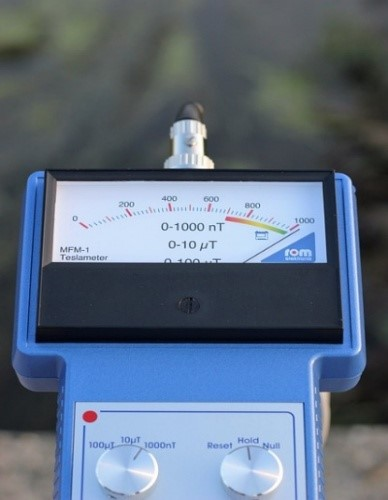
\includegraphics[width=0.7\linewidth]{img/magnometro.jpg}
	\caption{Sensor de proximidad}
	\label{fig:insertarimagen}
\end{figure}

\subsection{Fundamentos del Campo Magnético}

Para entender cómo funciona un magnetómetro, primero debemos comprender los conceptos básicos del campo magnético. Un campo magnético es una región del espacio donde una fuerza magnética actúa sobre materiales magnéticos o sobre partículas cargadas en movimiento. Los campos magnéticos son generados por corrientes eléctricas y por materiales magnéticos como los imanes.

\subsection{Tipos de Magnetómetros}

\begin{itemize}
    \item Magnetómetros de Inducción: Estos dispositivos miden los cambios en el flujo magnético a través de una bobina de alambre. Cuando un campo magnético variable atraviesa la bobina, induce una corriente eléctrica proporcional a la velocidad de cambio del campo.
    
    \item Magnetómetros de Protones (NMR): Utilizan el principio de resonancia magnética nuclear. En estos dispositivos, los protones en un fluido (generalmente agua) se alinean con un campo magnético externo. Cuando se retira el campo, los protones vuelven a su estado original, liberando energía en forma de una señal detectable.
    
    \item Magnetómetros de Efecto Hall: Basados en el efecto Hall, estos magnetómetros miden la tensión creada en un conductor por un campo magnético perpendicular a la corriente eléctrica que pasa a través del conductor.
    
    \item Magnetómetros SQUID (Dispositivos Superconductores de Interferencia Cuántica): Utilizan superconductores y el principio de interferencia cuántica para detectar campos magnéticos extremadamente débiles con una precisión muy alta.
    
\end{itemize}

\subsection{Funcionamiento Básico}

Independientemente del tipo, todos los magnetómetros tienen un principio común: detectan y miden la intensidad del campo magnético. Esto se logra mediante la interacción de los materiales dentro del magnetómetro con el campo magnético, generando una señal eléctrica que puede ser medida y analizada.

\subsection{Aplicaciones de los Magnetómetros}

\begin{itemize}
    \item Geofísica
    
    En geofísica, los magnetómetros se utilizan para mapear las variaciones en el campo magnético terrestre. Esto es crucial para la prospección minera, la detección de depósitos de minerales y la investigación geológica. Las anomalías magnéticas pueden indicar la presencia de diferentes tipos de rocas o minerales.
    
    \item Arqueología
    
    Los magnetómetros también son herramientas valiosas en arqueología. Pueden detectar estructuras subterráneas como muros, fosos y hornos antiguos, sin necesidad de excavar. Esto ayuda a los arqueólogos a identificar sitios de interés y planificar excavaciones de manera más eficiente.
    
    \item Física Espacial
     
    En el ámbito de la física espacial, los magnetómetros son fundamentales para estudiar los campos magnéticos de otros planetas y el espacio interplanetario. Los satélites y sondas espaciales equipados con magnetómetros pueden medir los campos magnéticos en el espacio, proporcionando información vital sobre el viento solar y las magnetósferas planetarias.
    
    \item Seguridad y Defensa

     En seguridad y defensa, los magnetómetros se utilizan para detectar submarinos y minas navales debido a las firmas magnéticas que estos objetos generan. También se emplean en la detección de dispositivos electrónicos y armas ocultas.
    
    
\end{itemize}

\subsection{¿Qué es un sensor LiDAR}

Un Sensor LiDAR, del acrónimo LiDAR (en inglés, Light Detection and Ranging o Laser Imaging Detection and Ranging) es un sistema de medición y detección de objetos a través del láser. En otras palabras: una tecnología de escaneo y teledetección que utiliza la emisión de un pulso de láser para calcular superficies y mapear espacios en tres dimensiones (3D).


\begin{figure}[h]
	\centering
	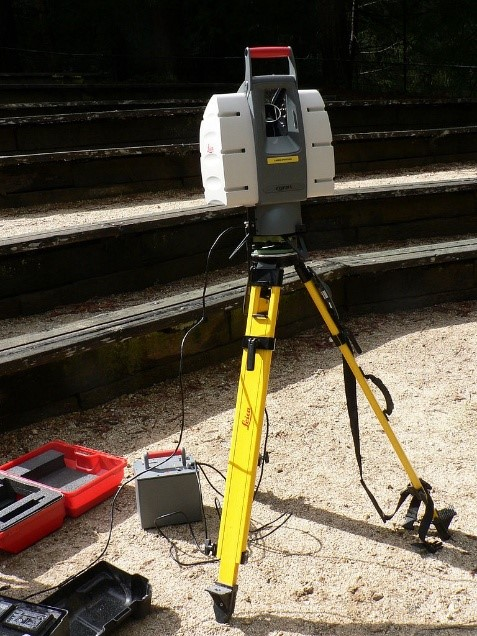
\includegraphics[width=0.7\linewidth]{img/LIDAR.jpg}
	\caption{Sensor lidar}
	\label{fig:insertarimagen}
\end{figure}

Existen tres tipos básico de sensores LiDAR:

\begin{itemize}
    \item Aerotransportado; se utiliza desde un helicóptero, avión o drone, en donde el láser se pulsa a través del aire y la vegetación.
     \item Terrestre: pueden ser móviles, en caso se usen desde vehículos en movimiento, y estacionarios.
    \item Acuático: láser barimétrico, usado para recopilar tanto la profundidad como elevación del agua y que es utilizado en el estudio de fondos marinos.
\end{itemize}

Adicionalmente, están compuesto por tres elementos esenciales:

\begin{itemize}
    \item Escáner láser, el cual sirve para medir distancias y ángulo.
    \item Sistemas de navegación y posicionamiento tales como el GPS (Global positioning system, Sistema de posicionamiento global) e INS (Inertial navigation system, Sistema de navegación inercial), debido a que es sumamente importante que la posición y orientación del sensor confirmen que los datos capturados son datos utilizables.
    \item Tecnología informativa, la cual sirve para procesar y aprovechar los datos recogidos.
    \item 
\end{itemize}

 \subsection{¿Cómo funciona un sensor LiDAR?}

En primera instancia, el escáner emite rayos láser infrarrojos que impactan sobre determinados objetos y rebotan. Posteriormente, aquellos rayos que “regresan” son registrados por un receptor y se realiza una medición de la distancia (tiempo de viaje x velocidad de la luz). Vale mencionar que un LiDAR dispara miles de rayos por segundo, los cuales generan la llamada “nube de puntos” (colecciones de puntos de elevación), la cual se combina con información posicional GPS/INS y genera un mapa de puntos tridimensionales reales.

Asimismo, el LiDAR se clasifica en dos categorías: por tipo de láser y por tipo de escaneado. Con relación al tipo de láser, el sensor puede presentar LiDAR de pulsos (en el cual el proceso de medición se lleva a cabo mediante el cálculo del tiempo en que tarda un pulso desde que es emitido y hasta que es captado por el receptor) y LiDAR de medición de fase (el número de longitud de ondas enteras recorridas que resulta de la diferencia de fase entre señales emitidas y reflejadas).
El tipo de escaneado presente en los LiDAR, por su parte, puede tomar cuatro formas: a modo de líneas (se producen líneas paralelas al momento de realizar el escaneado debido a que el sensor posee un espejo rotatorio que desvía el haz láser), zizgag (el espejo rotatorio produce líneas en forma de zigzag como patrón de escaneado debido a que el espejo es rotatorio en dos sentidos, ida y vuelta), fibra óptica (el haz láser es desviado desde un cable de fibra óptica, y el patrón de escaneado toma la forma de pequeñas circunferencias) y elíptica (el patrón de escaneado toma forma elíptica, el cual se produce a través del desvío del haz láser por intermedio de dos espejos).

Esta tecnología ha sido aplicada en múltiples campos que hacen uso de labores de mapeo, tales como:

\begin{itemize}
    \item Agricultura: exploración y estudio de la estructura del suelo, con lo cual se permite identificar qué especies son idóneas para el cultivo.
    \item Topografía: creación de ortofotos o fotografías de determinadas áreas de la superficie terrestre, determinación del uso de la tierra e investigación de deslizamientos de tierra.
    \item Arqueología: detección de vestigios y ciudades ocultas escondidas bajo la vegetación.
    \item Ciencias forenses: reconstrucción de escenas del crimen y detección de zonas de entierro de cadáveres debido a la presencia de anomalías en la tierra.
    \item Fotografía: su inclusión en los últimos modelos del iPhone Pro causó sensación, ya que ayudó a que las funciones de realidad aumentada y de fotografía de dicho teléfono fueran más especializadas y ayudaran a mejorar la experiencia de los usuarios.
    \item Meteorología: medición y monitorización de fenómenos atmosféricos y calidad del aire.
    \item Ambito automotriz: en aquellos autos que poseen modo de piloto automático, el sensor ayuda a detectar la naturaleza y proximidad de objetos que circunden el vehículo. Esto permite que el auto no requiera de un sujeto que lo maneje, lo que también ayuda a disminuir el número de accidentes de tráfico.
\end{itemize}

\subsection{¿Cuáles son las ventajas que proporciona?}

En primer lugar, este sensor puede funcionar por sí solo o de manera autónoma y no depende exclusivamente de la interacción con un ser humano. Este hecho implica un ahorro significativo de tiempo y esfuerzo. En segundo lugar, permite crear modelos en tres dimensiones (a diferencia de la fotogrametría, por ejemplo, que solo es capaz de crear modelos basados en imágenes bidimensionales), los cuales recogen información que involucra densidad de superficies. También recopila datos precisos de forma instantánea gracias al uso del láser, lo cual contribuye a agilizar procesos.


\cite{acelerometro}
\cite{acelerometro_wikipedia}
\cite{giroscopio}
\cite{lidar}
\cite{magnetometro}
\cite{piezo_switch}
\cite{potenciometros_rotativos}
\cite{sensor_aeroexpo}
\cite{sensor_angulo}
\cite{sensor_efecto_hall}
\cite{sensor_gps_campbellsci}
\cite{sensor_gps_neo6m}
\cite{sensor_magnetostrictivo}
\cite{sensor_posicion_cd18}
\cite{sensor_posicion_elegir}
\cite{sensor_posicion_potenciometrico}
\cite{sensores_actuadores}
\cite{sensores_lineales}
\cite{sensores_proximidad}
\cite{sensores_robot_industrial}
\cite{sensores_velocidad}
\cite{sistema_sensorial}
\cite{tacometro_peak_meter}
\cite{tacometro_rentingfinders}

Repositorio: https://github.com/MFVM231/Robotica1.git














\section{Ecuaciones}
Para realizar ecuaciones, se pueden ayudar mucho de ChatGPT (Como copiar una imagen y que lea la ecuación para dártela en formato \LaTeX) y de que MATLAB, word y algunas páginas te permiten copiar ecuaciones en formato \LaTeX. El modelo en espacio de estados de un robot de dos grados de libertad, el cual se puede ver en el Capítulo 5: Dinámica del Robot en \cite{barrientos2007fundamentos} se expresa como

\begin{equation}
	\label{eq:spaceStateRobot}
	\begin{bmatrix}
		\dot{q} \\
		\ddot{q}
	\end{bmatrix} =
	\begin{bmatrix}
		0 & I \\
		M^{-1}(-C - G)
	\end{bmatrix}
	\begin{bmatrix}
		q \\
		\dot{q}
	\end{bmatrix} +
	\begin{bmatrix}
		0 \\
		M^{-1} B
	\end{bmatrix} u,
\end{equation}
donde:
\begin{itemize}
	\item \( q \) es el vector de posiciones articulares del robot.
	\item \( \dot{q} \) y \( \ddot{q} \) son las velocidades y aceleraciones articulares.
	\item \( M \) es la matriz de inercia.
	\item \( C \) representa las fuerzas centrífugas y de Coriolis.
	\item \( G \) es el vector de fuerzas gravitacionales.
	\item \( B \) es la matriz de entrada de los torques.
	\item \( u \) es el vector de torques aplicados a las articulaciones.
\end{itemize}

Cabe destacar que en \eqref{eq:spaceStateRobot}, la ecuación se referencia después de haberla nombrado y forma parte de la oración, por lo que debe llevar puntos o comas. También al referenciar, debe de estar entre paréntesis con \texttt{eqref}.
\section{Conclusión} \label{sec:conclusion}
Los sensores internos y externos son fundamentales en la recopilación de datos y el monitoreo de sistemas, diferenciándose por su ubicación y las variables que miden. Los sensores internos se encuentran dentro de un dispositivo o sistema, supervisando condiciones internas como temperatura, presión o voltaje, y son clave para asegurar el correcto funcionamiento y estabilidad de equipos, como motores o baterías. Por otro lado, los sensores externos están ubicados fuera del sistema y se utilizan para detectar estímulos en el entorno, como proximidad, movimiento o gases, y son esenciales en aplicaciones como seguridad, monitoreo ambiental o control de procesos industriales. Ambos tipos trabajan en conjunto para crear sistemas más eficientes, inteligentes y seguros, mejorando la interacción con el entorno y optimizando el rendimiento.


%-------------------------------------------
% Bibliografía
%-------------------------------------------
\bibliographystyle{IEEEtran}  % Estilo de bibliografía IEEE
% La bibliografía se tomará del archivo "fuentes.bib"
\bibliography{fuentes}
	
\end{document}
